\chapter{Kantorovich 問題}
\label{ch:sem-kantorovich-chapter}

\subsection{Kantorovich 緩和}
\label{sec:sem-kantorovich}

\subsubsection{問題の定義}

\begin{definition}{Kantorovich 問題}{sem-kantorovich}
\blockmeta{space=polish}
  $\X, \Y$ 上の確率測度（定義~\ref{def:sem-probability-measure}）$\alpha \in \Mm_+^1(\X)$, $\beta \in \Mm_+^1(\Y)$ と
  可測関数 $c \colon \X \times \Y \to \Rnn$ に対して，
  \textbf{カップリング集合}
  \[
    \Couplings(\alpha, \beta) \defeq
    \left\{ \pi \in \Mm_+^1(\X \times \Y) \;\middle|\;
      \begin{aligned}
        &\pi(A \times \Y) = \alpha(A) \quad \forall\, A \in \Bb(\X), \\
        &\pi(\X \times B) = \beta(B)  \quad \forall\, B \in \Bb(\Y)
      \end{aligned}
    \right\}
  \]
  上で輸送コスト
  \[
    \MK_c(\alpha, \beta) \defeq
    \inf_{\pi \in \Couplings(\alpha, \beta)}
    \int_{\X \times \Y} c(x, y) \, \d\pi(x, y)
  \]
  を最小化する問題を\textbf{Kantorovich 問題}という．
\end{definition}

\begin{remark}{押し出しを用いたコンパクトな表現}{sem-marginal-pushforward}
  カップリング条件は，射影（定義~\ref{def:sem-projection}）
  $P_\X \colon (x,y) \mapsto x$，$P_\Y \colon (x,y) \mapsto y$ と
  押し出し（定義~\ref{def:sem-pushforward}）を用いると
  \[
    (P_\X)\pushforward \pi = \alpha, \qquad (P_\Y)\pushforward \pi = \beta
  \]
  とコンパクトに書ける．実際，任意の $A \in \Bb(\X)$ に対して
  \[
    \bigl((P_\X)\pushforward \pi\bigr)(A)
    = \pi\bigl(P_\X^{-1}(A)\bigr)
    = \pi\bigl(\{(x,y) \mid x \in A\}\bigr)
    = \pi(A \times \Y),
  \]
  ゆえに $(P_\X)\pushforward \pi = \alpha$ は
  $\pi(A \times \Y) = \alpha(A)$（$\forall\, A \in \Bb(\X)$）と同値である．
  $P_\Y$ についても同様．
\end{remark}

\begin{figure}[H]
\centering
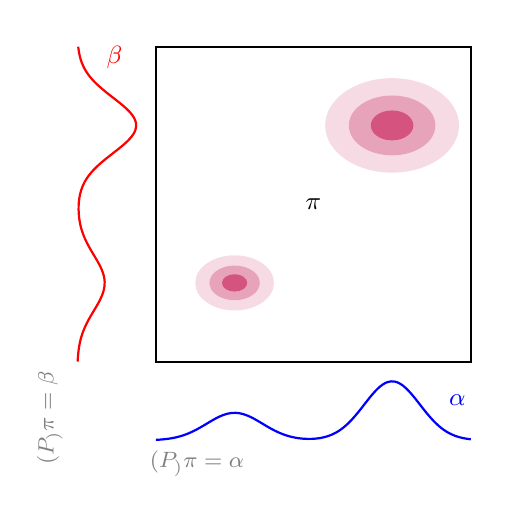
\begin{tikzpicture}[scale=1.0]
  % --- 正方形 X × Y ---
  \draw[thick] (0, 0) rectangle (4, 4);
  \node[font=\small, below right] at (4, 0) {$\X$};
  \node[font=\small, above left] at (0, 4) {$\Y$};

  % --- π を表す 2 つの集中領域（紫の濃淡，サイズで重みを表現）---
  % 小さい山: (1, 1) ; 大きい山: (3, 3)
  \fill[purple!20, opacity=0.7] (1.0, 1.0) ellipse (0.5 and 0.35);
  \fill[purple!45, opacity=0.7] (1.0, 1.0) ellipse (0.32 and 0.22);
  \fill[purple!75, opacity=0.8] (1.0, 1.0) ellipse (0.16 and 0.11);
  \fill[purple!20, opacity=0.7] (3.0, 3.0) ellipse (0.85 and 0.6);
  \fill[purple!45, opacity=0.7] (3.0, 3.0) ellipse (0.55 and 0.38);
  \fill[purple!75, opacity=0.8] (3.0, 3.0) ellipse (0.27 and 0.19);
  \node[font=\small] at (2.0, 2.0) {$\pi$};

  % --- α: X への射影（下方，2 山の密度曲線；高さ非対称） ---
  \draw[blue, thick, smooth, samples=80, domain=0:4]
    plot (\x, {-1 + 0.35*exp(-(\x-1.0)*(\x-1.0)*4)
                + 0.75*exp(-(\x-3.0)*(\x-3.0)*4)});
  \node[blue, font=\small, anchor=north west] at (3.6, -0.3) {$\alpha$};
  \node[font=\footnotesize, gray, anchor=west] at (-0.2, -1.3)
    {$(P_\X)\pushforward \pi = \alpha$};

  % --- β: Y への射影（左方，2 山の密度曲線；高さ非対称） ---
  \draw[red, thick, smooth, samples=80, domain=0:4, variable=\y]
    plot ({-1 + 0.35*exp(-(\y-1.0)*(\y-1.0)*4)
            + 0.75*exp(-(\y-3.0)*(\y-3.0)*4)}, \y);
  \node[red, font=\small, anchor=south east] at (-0.3, 3.6) {$\beta$};
  \node[font=\footnotesize, gray, anchor=base east, rotate=90] at (-1.3, 0.0)
    {$(P_\Y)\pushforward \pi = \beta$};
\end{tikzpicture}
\caption{カップリング $\pi \in \Couplings(\alpha, \beta)$ の概念図．
$\X \times \Y$ 上に分布する $\pi$（中央の紫領域）について，
$\X$ への射影が $\alpha$，$\Y$ への射影が $\beta$ に一致する．}
\label{fig:sem-coupling-continuous}
\end{figure}

\begin{figure}[htbp]
\centering
\begin{tikzpicture}[scale=0.95]
  % Monge (left)
  \node[above] at (1.5, 3.3) {\textbf{Monge 写像}};
  \fill[blue] (0.5, 2.5) circle (3pt) node[left] {\small $x_1$};
  \fill[blue] (0.5, 1.5) circle (3pt) node[left] {\small $x_2$};
  \fill[blue] (0.5, 0.5) circle (3pt) node[left] {\small $x_3$};
  \fill[red] (2.5, 2.5) circle (3pt) node[right] {\small $y_1$};
  \fill[red] (2.5, 1.5) circle (3pt) node[right] {\small $y_2$};
  \draw[->, thick] (0.7, 2.5) -- (2.3, 2.5);
  \draw[->, thick] (0.7, 1.5) -- (2.3, 2.5);
  \draw[->, thick] (0.7, 0.5) -- (2.3, 1.5);
  \node[below, text width=3cm, align=center] at (1.5, -0.2) {\small 各点は1つの\\行き先のみ};

  % Kantorovich (right)
  \begin{scope}[xshift=5.5cm]
    \node[above] at (1.5, 3.3) {\textbf{Kantorovich カップリング}};
    \fill[blue] (0.5, 2.5) circle (3pt) node[left] {\small $x_1$};
    \fill[blue] (0.5, 1.5) circle (3pt) node[left] {\small $x_2$};
    \fill[blue] (0.5, 0.5) circle (3pt) node[left] {\small $x_3$};
    \fill[red] (2.5, 2.5) circle (3pt) node[right] {\small $y_1$};
    \fill[red] (2.5, 1.5) circle (3pt) node[right] {\small $y_2$};
    \draw[->, thick] (0.7, 2.5) -- (2.3, 2.5);
    \draw[->, thick, blue!60] (0.7, 1.5) -- (2.3, 2.5);
    \draw[->, thick, red!60] (0.7, 1.5) -- (2.3, 1.5);
    \draw[->, thick] (0.7, 0.5) -- (2.3, 1.5);
    \node[right, font=\small] at (1.6, 1.8) {分割};
    \node[below, text width=3cm, align=center] at (1.5, -0.2) {\small 質量の分割を\\許す};
  \end{scope}
\end{tikzpicture}
\caption{Monge 写像と Kantorovich カップリングの対比．Monge 写像は各点を1つの行き先に送るが，Kantorovich カップリングは質量の分割を許す．}
\label{fig:sem-monge-vs-kantorovich}
\end{figure}

\subsubsection{離散化}

連続定義~\ref{def:sem-kantorovich}に
定義~\ref{def:sem-discrete-measure}を代入すると，次の命題が示すとおり行列最適化へ帰着する．

\begin{proposition}{連続 Kantorovich 問題の離散化}{sem-discrete-kantorovich}
  $\mathbf{a} \in \Rpos^n$（$\sum_i a_i = 1$），$\mathbf{b} \in \Rpos^m$（$\sum_j b_j = 1$），
  $x_1, \ldots, x_n \in \X$（$i \neq j \Rightarrow x_i \neq x_j$），
  $y_1, \ldots, y_m \in \Y$（$i \neq j \Rightarrow y_i \neq y_j$），
  可測関数 $c \colon \X \times \Y \to \Rnn$ を所与とし，
  \[
    \alpha \defeq \sum_{i=1}^n a_i\, \delta_{x_i} \in \Mm_+^1(\X), \qquad
    \beta  \defeq \sum_{j=1}^m b_j\, \delta_{y_j} \in \Mm_+^1(\Y)
  \]
  とおく．行列 $\mathbf{C} \defeq \bigl(c(x_i, y_j)\bigr)_{i,j} \in \Rnn^{n \times m}$ および
  \textbf{離散カップリング集合}
  \[
    \CouplingsD(\mathbf{a}, \mathbf{b}) \defeq
    \left\{ \mathbf{P} \in \Rnn^{n \times m} \;\middle|\;
      \mathbf{P}\ones_m = \mathbf{a},\;
      \mathbf{P}^\top\ones_n = \mathbf{b}
    \right\}
  \]
  に対して
  \[
    \inf_{\pi \in \Couplings(\alpha,\beta)}
      \int_{\X\times\Y} c\,\d\pi
    = \inf_{\mathbf{P} \in \CouplingsD(\mathbf{a}, \mathbf{b})}
      \inner{\mathbf{C}}{\mathbf{P}}
  \]
  が成り立つ．ここで $\ones_m, \ones_n$ は全成分 $1$ のベクトル（定義~\ref{def:sem-ones-vector}），
  $\inner{\mathbf{C}}{\mathbf{P}} \defeq \sum_{i,j} C_{i,j} P_{i,j}$ はフロベニウス内積
  （定義~\ref{def:sem-frobenius-inner}）である．
\end{proposition}
\begin{proof}
  次の 2 点を示す：
  \begin{itemize}
    \item[(A)] 全単射 $\varphi \colon \Couplings(\alpha,\beta) \xrightarrow{\sim} \CouplingsD(\mathbf{a},\mathbf{b})$
      が存在する（(A-1) $\varphi$ の構成，(A-2) 値域の確認，(A-3) 全射性，(A-4) 単射性）．
    \item[(B)] $\varphi$ はコストを保存する：
      $\displaystyle\int_{\X\times\Y} c\,\d\pi = \inner{\mathbf{C}}{\varphi(\pi)}$．
  \end{itemize}
  \medskip
  \textbf{(A-1) $\varphi$ の構成．}
  任意の $\pi \in \Couplings(\alpha, \beta)$ をとる．
  周辺条件 $\pi(A \times \Y) = \alpha(A)$（$\forall A \in \Bb(\X)$）と
  $\alpha(\X \setminus \{x_1,\ldots,x_n\}) = 0$ から
  \[
    \pi\bigl((\X \setminus \{x_1,\ldots,x_n\}) \times \Y\bigr) = 0,
  \]
  同様に $\pi(\X \times (\Y \setminus \{y_1,\ldots,y_m\})) = 0$．
  測度の劣加法性から
  \[
    \pi\bigl((\X\times\Y)\setminus(\{x_1,\ldots,x_n\}\times\{y_1,\ldots,y_m\})\bigr)
    \;\leq\;
    \pi\bigl((\X\setminus\{x_1,\ldots,x_n\})\times\Y\bigr)
    + \pi\bigl(\X\times(\Y\setminus\{y_1,\ldots,y_m\})\bigr) = 0.
  \]
  よって $\pi$ は有限格子 $\{x_1,\ldots,x_n\} \times \{y_1,\ldots,y_m\}$ 上のみに質量を持ち，
  \[
    \varphi(\pi)_{i,j} \defeq P_{i,j} \defeq \pi\bigl(\{x_i\} \times \{y_j\}\bigr) \geq 0
  \]
  と定めると $\pi = \sum_{i,j} P_{i,j}\, \delta_{(x_i, y_j)}$ と書ける．

  \medskip
  \textbf{(A-2) $\varphi(\pi) \in \CouplingsD(\mathbf{a},\mathbf{b})$（周辺条件 $\leftrightarrow$ 行・列和条件）．}
  任意の $k$ に対し，
  \[
    \sum_{j=1}^m P_{k,j}
    = \sum_{j=1}^m \pi\bigl(\{x_k\} \times \{y_j\}\bigr)
    = \pi\!\left(\{x_k\} \times \{y_1,\ldots,y_m\}\right)
    = \pi(\{x_k\} \times \Y)
    = \alpha(\{x_k\}) = a_k.
  \]
  第二の等号は $\{y_j\}$ が互いに素であることによる $\sigma$-加法性，
  第三の等号は (A-1) より $\pi$ の質量が格子上のみに集中することによる．
  ゆえに $\mathbf{P}\ones_m = \mathbf{a}$．
  同様に $\pi(\X \times \{y_l\}) = \beta(\{y_l\}) = b_l$ から $\mathbf{P}^\top\ones_n = \mathbf{b}$．
  ゆえに $\mathbf{P} \in \CouplingsD(\mathbf{a},\mathbf{b})$．

  \medskip
  \textbf{(A-3) 全射性．}
  任意の $\mathbf{P} \in \CouplingsD(\mathbf{a},\mathbf{b})$ に対し
  $\pi' \defeq \sum_{i,j} P_{i,j}\,\delta_{(x_i,y_j)}$ とおくと，
  任意の $A \in \Bb(\X)$ について
  \[
    \pi'(A \times \Y)
    = \sum_{i:\,x_i \in A} \sum_j P_{i,j}
    = \sum_{i:\,x_i \in A} a_i
    = \alpha(A),
  \]
  同様に $\pi'(\X \times B) = \beta(B)$（$\forall B \in \Bb(\Y)$）だから
  $\pi' \in \Couplings(\alpha,\beta)$．
  また $\varphi(\pi')_{i,j} = \pi'(\{x_i\} \times \{y_j\})$ に $\pi' = \sum_{k,l} P_{k,l}\,\delta_{(x_k,y_l)}$ を代入すると，
  \[
    \pi'(\{x_i\} \times \{y_j\})
    = \sum_{k,l} P_{k,l}\,\delta_{(x_k,y_l)}(\{x_i\} \times \{y_j\})
    = P_{i,j}.
  \]
  最後の等号は，$x_k$ はすべて互いに異なり $y_l$ もすべて互いに異なるという仮定より，$\delta_{(x_k,y_l)}(\{x_i\}\times\{y_j\})=1$ となるのは $(k,l)=(i,j)$ のときに限ることによる．
  ゆえに $\varphi(\pi') = \mathbf{P}$ であり，任意の $\mathbf{P} \in \CouplingsD(\mathbf{a},\mathbf{b})$ に対して $\varphi(\pi') = \mathbf{P}$ を満たす $\pi' \in \Couplings(\alpha,\beta)$ が存在するから，$\varphi$ は全射である．

  \medskip
  \textbf{(A-4) 単射性．}
  任意の $\pi \in \Couplings(\alpha,\beta)$ をとり $\mathbf{P} \defeq \varphi(\pi)$ とおくと，
  (A-1) より
  \[
    \pi = \sum_{i,j} P_{i,j}\,\delta_{(x_i,y_j)}
  \]
  と一意に表せる．ゆえに $\varphi(\pi)$ が等しければ $\pi$ も等しく，$\varphi$ は単射である．

  \medskip
  \textbf{(B) $\varphi$ はコストを保存する．}
  任意の $\pi \in \Couplings(\alpha,\beta)$ をとり $\mathbf{P} \defeq \varphi(\pi)$ とおく．
  (A-1) より $\pi = \sum_{i,j} P_{i,j}\,\delta_{(x_i,y_j)}$ だから，
  積分の線形性（命題~\ref{prop:sem-measure-linearity}）を適用すると
  \[
    \int_{\X \times \Y} c(x, y)\, \d\pi(x, y)
    = \sum_{i,j} P_{i,j} \int_{\X \times \Y} c(x, y)\, \d\delta_{(x_i,y_j)}(x,y).
  \]
  Dirac 測度に対する積分（主張~\ref{clm:sem-dirac-integral}）より
  $\int c\,\d\delta_{(x_i,y_j)} = c(x_i,y_j) = C_{i,j}$ だから，
  \[
    \int_{\X \times \Y} c(x, y)\, \d\pi(x, y)
    = \sum_{i,j} P_{i,j}\, C_{i,j}
    = \inner{\mathbf{C}}{\mathbf{P}}.
  \]

  \medskip
  \textbf{結論．}
  (A)(B) より $\varphi$ はコストを保存する全単射だから，
  \[
    \MK_c(\alpha, \beta)
    = \inf_{\pi \in \Couplings(\alpha, \beta)}
      \int_{\X \times \Y} c\, \d\pi
    = \inf_{\mathbf{P} \in \CouplingsD(\mathbf{a}, \mathbf{b})}
      \inner{\mathbf{C}}{\mathbf{P}}.
  \]
\end{proof}

右辺の最適値を
\[
  \MKD_{\mathbf{C}}(\mathbf{a}, \mathbf{b})
  \defeq \inf_{\mathbf{P} \in \CouplingsD(\mathbf{a}, \mathbf{b})} \inner{\mathbf{C}}{\mathbf{P}}
\]
と書き，\textbf{離散 Kantorovich 問題}と呼ぶ．

\begin{remark}{相異性条件の必要性}{sem-distinct-points}
  命題の仮定「$i \neq j \Rightarrow x_i \neq x_j$」は全単射 $\varphi$ の全射性に本質的である．
  もし $x_i = x_k$（$i \neq k$）であれば，$\varphi(\pi)_{i,j} = \varphi(\pi)_{k,j} = \pi(\{x_i\} \times \{y_j\})$
  となり，$\varphi$ の値域は常に $P_{i,j} = P_{k,j}$ を満たす行列に限定される．
  一方 $\CouplingsD(\mathbf{a}, \mathbf{b})$ には $P_{i,j} \neq P_{k,j}$ な行列が存在するため，
  $\varphi$ は全射とならず命題の等式が崩れる．
  なお，重複点を統合すれば（$a_i + a_k$ をまとめた）より小さい次元の多面体との全単射が取れるため，
  離散 Kantorovich 問題の枠組み自体は相異性なしでも成立する．
\end{remark}

\begin{example}{工場からスーパーへの輸送}{sem-factory-supermarket}
  2 つの工場 $x_1, x_2$ から 2 つのスーパー $y_1, y_2$ へ商品を輸送する状況を考える．
  各工場の供給割合を $\mathbf{a} = (2/3,\; 1/3)^\top$，
  各スーパーの需要割合を $\mathbf{b} = (1/3,\; 2/3)^\top$ とし，
  輸送コスト行列を
  \[
    \mathbf{C} =
    \begin{pmatrix}
      C_{1,1} & C_{1,2} \\
      C_{2,1} & C_{2,2}
    \end{pmatrix}
    =
    \begin{pmatrix}
      1 & 2 \\
      3 & 1
    \end{pmatrix}
  \]
  とする（図~\ref{fig:sem-factory-supermarket-cost}）．

  \begin{figure}[H]
    \centering
    \begin{tikzpicture}[
      factory/.style={draw, fill=blue!15, rounded corners, minimum width=1.6cm, minimum height=0.9cm},
      super/.style={draw, fill=orange!15, rounded corners, minimum width=1.6cm, minimum height=0.9cm},
      every edge/.style={draw, -{Stealth[length=5pt]}, thick},
      cost label/.style={font=\small, fill=white, inner sep=1.5pt},
    ]
      % 工場ノード
      \node[factory] (x1) at (0, 1.5) {$x_1$};
      \node[factory] (x2) at (0, -1.5) {$x_2$};
      % スーパーノード
      \node[super] (y1) at (5, 1.5) {$y_1$};
      \node[super] (y2) at (5, -1.5) {$y_2$};
      % 供給・需要ラベル
      \node[left=0.3cm of x1, font=\small] {$a_1 = \tfrac{2}{3}$};
      \node[left=0.3cm of x2, font=\small] {$a_2 = \tfrac{1}{3}$};
      \node[right=0.3cm of y1, font=\small] {$b_1 = \tfrac{1}{3}$};
      \node[right=0.3cm of y2, font=\small] {$b_2 = \tfrac{2}{3}$};
      % コスト辺
      \draw (x1) edge node[cost label, pos=0.5, above] {$C_{1,1}=1$} (y1);
      \draw (x1) edge node[cost label, pos=0.35, below] {$C_{1,2}=2$} (y2);
      \draw (x2) edge node[cost label, pos=0.35, above] {$C_{2,1}=3$} (y1);
      \draw (x2) edge node[cost label, pos=0.5, below] {$C_{2,2}=1$} (y2);
      % ラベル
      \node[above=0.3cm of x1, font=\small\bfseries] {工場};
      \node[above=0.3cm of y1, font=\small\bfseries] {スーパー};
    \end{tikzpicture}
    \caption{輸送コストのネットワーク．各辺の数値は単位量あたりの輸送コスト $C_{i,j}$ を表す．}
    \label{fig:sem-factory-supermarket-cost}
  \end{figure}

  コストの安い経路 $x_1 \to y_1$（コスト $1$）と $x_2 \to y_2$（コスト $1$）を
  最大限利用し，残りを $x_1 \to y_2$（コスト $2$）で補うのが最適であり，
  \[
    \mathbf{P}^{\star} =
    \begin{pmatrix}
      1/3 & 1/3 \\
      0 & 1/3
    \end{pmatrix}.
  \]

  $\mathbf{P}^{\star} \in \CouplingsD(\mathbf{a}, \mathbf{b})$ であることを周辺条件から確認する：
  \[
    \mathbf{P}^{\star}\ones_2
    = \begin{pmatrix} \tfrac{1}{3} + \tfrac{1}{3} \\ 0 + \tfrac{1}{3} \end{pmatrix}
    = \begin{pmatrix} \tfrac{2}{3} \\ \tfrac{1}{3} \end{pmatrix}
    = \mathbf{a},
    \qquad
    (\mathbf{P}^{\star})^\top\ones_2
    = \begin{pmatrix} \tfrac{1}{3} + 0 \\ \tfrac{1}{3} + \tfrac{1}{3} \end{pmatrix}
    = \begin{pmatrix} \tfrac{1}{3} \\ \tfrac{2}{3} \end{pmatrix}
    = \mathbf{b}.
  \]


  最適コストは
  \[
    \MKD_{\mathbf{C}}(\mathbf{a}, \mathbf{b})
    = \inner{\mathbf{C}}{\mathbf{P}^{\star}}
    = \sum_{i,j} C_{i,j} P_{i,j}^{\star}
    = 1 \cdot \tfrac{1}{3} + 2 \cdot \tfrac{1}{3} + 3 \cdot 0 + 1 \cdot \tfrac{1}{3}
    = \tfrac{4}{3}.
  \]

  \begin{figure}[H]
    \centering
    \begin{tikzpicture}[
      factory/.style={draw, fill=blue!15, rounded corners, minimum width=1.6cm, minimum height=0.9cm},
      super/.style={draw, fill=orange!15, rounded corners, minimum width=1.6cm, minimum height=0.9cm},
      every edge/.style={draw, -{Stealth[length=5pt]}},
      cost label/.style={font=\small, fill=white, inner sep=1.5pt},
    ]
      % 工場ノード
      \node[factory] (x1) at (0, 1.5) {$x_1$};
      \node[factory] (x2) at (0, -1.5) {$x_2$};
      % スーパーノード
      \node[super] (y1) at (5, 1.5) {$y_1$};
      \node[super] (y2) at (5, -1.5) {$y_2$};
      % 供給・需要ラベル
      \node[left=0.3cm of x1, font=\small] {$a_1 = \tfrac{2}{3}$};
      \node[left=0.3cm of x2, font=\small] {$a_2 = \tfrac{1}{3}$};
      \node[right=0.3cm of y1, font=\small] {$b_1 = \tfrac{1}{3}$};
      \node[right=0.3cm of y2, font=\small] {$b_2 = \tfrac{2}{3}$};
      % 最適輸送の辺（太さで量を表現，コスト併記）
      \draw[line width=2.0pt, blue!70] (x1) edge node[cost label, above] {$P_{1,1}^{\star}=\tfrac{1}{3}$\;\scriptsize$(C=1)$} (y1);
      \draw[line width=2.0pt, blue!70] (x1) edge node[cost label, pos=0.35, below] {$P_{1,2}^{\star}=\tfrac{1}{3}$\;\scriptsize$(C=2)$} (y2);
      \draw[line width=0.4pt, gray, dashed] (x2) edge node[cost label, pos=0.35, above, text=gray] {$P_{2,1}^{\star}=0$\;\scriptsize$(C=3)$} (y1);
      \draw[line width=2.0pt, blue!70] (x2) edge node[cost label, below] {$P_{2,2}^{\star}=\tfrac{1}{3}$\;\scriptsize$(C=1)$} (y2);
      % ラベル
      \node[above=0.3cm of x1, font=\small\bfseries] {工場};
      \node[above=0.3cm of y1, font=\small\bfseries] {スーパー};
    \end{tikzpicture}
    \caption{最適輸送計画 $\mathbf{P}^{\star}$．
    安価な経路 $x_1 \to y_1$（コスト $1$）と $x_2 \to y_2$（コスト $1$）を
    最大限利用し，残りを $x_1 \to y_2$（コスト $2$）で補う．
    高コストの $x_2 \to y_1$（コスト $3$）は使われない．}
    \label{fig:sem-factory-supermarket-opt}
  \end{figure}
\end{example}


\begin{figure}[H]
\centering
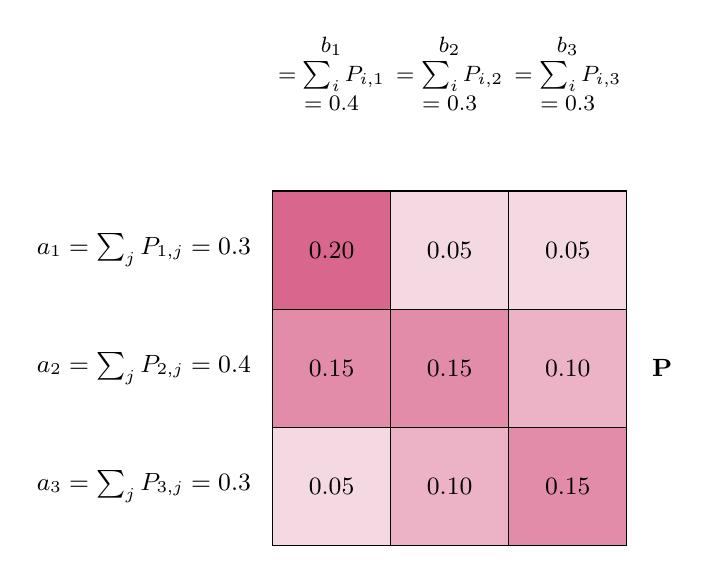
\begin{tikzpicture}[scale=1.0]
  % ---- 上ヘッダー: b_j = sum_i P_{i,j} = value（3 行に折りたたみ） ----
  \node[font=\footnotesize, anchor=south, align=center] at (1.5, 0.15)
    {$b_1$ \\[1pt] $= \textstyle\sum_i P_{i,1}$ \\[1pt] $= 0.4$};
  \node[font=\footnotesize, anchor=south, align=center] at (3.0, 0.15)
    {$b_2$ \\[1pt] $= \textstyle\sum_i P_{i,2}$ \\[1pt] $= 0.3$};
  \node[font=\footnotesize, anchor=south, align=center] at (4.5, 0.15)
    {$b_3$ \\[1pt] $= \textstyle\sum_i P_{i,3}$ \\[1pt] $= 0.3$};

  % ---- 左ヘッダー: a_i = sum_j P_{i,j} = value（1 行） ----
  \node[font=\small, anchor=east] at (0.6, -1.5) {$a_1 = \sum_j P_{1,j} = 0.3$};
  \node[font=\small, anchor=east] at (0.6, -3.0) {$a_2 = \sum_j P_{2,j} = 0.4$};
  \node[font=\small, anchor=east] at (0.6, -4.5) {$a_3 = \sum_j P_{3,j} = 0.3$};

  % ---- 行列 P （3x3） ----
  \foreach \i/\j/\v/\op in {%
    1/1/0.20/60, 1/2/0.05/15, 1/3/0.05/15,%
    2/1/0.15/45, 2/2/0.15/45, 2/3/0.10/30,%
    3/1/0.05/15, 3/2/0.10/30, 3/3/0.15/45}{%
    \fill[purple!\op] (1.5*\j - 0.75, -1.5*\i + 0.75)
                      rectangle (1.5*\j + 0.75, -1.5*\i - 0.75);
    \draw (1.5*\j - 0.75, -1.5*\i + 0.75)
          rectangle (1.5*\j + 0.75, -1.5*\i - 0.75);
    \node[font=\small] at (1.5*\j, -1.5*\i) {$\v$};
  }

  % ---- P ラベル ----
  \node[font=\small\bfseries] at (5.7, -3.0) {$\mathbf{P}$};
\end{tikzpicture}
\caption{離散カップリング $\mathbf{P} \in \CouplingsD(\mathbf{a}, \mathbf{b})$ の構造．
中央の $3 \times 3$ 行列が $\mathbf{P}$（色の濃さが値 $P_{i,j}$ の大きさを表す）．}
\label{fig:sem-coupling-matrix}
\end{figure}

\subsubsection{最適解の存在と性質}

\begin{claim}{離散 Kantorovich 問題の解の存在}{sem-discrete-kantorovich-existence}
  任意の $\mathbf{a} \in \Rpos^n$，$\mathbf{b} \in \Rpos^m$
  （$\sum_i a_i = \sum_j b_j = 1$）と $\mathbf{C} \in \Rnn^{n \times m}$ に対して，
  \[
    \MKD_{\mathbf{C}}(\mathbf{a}, \mathbf{b}) = \inner{\mathbf{C}}{\mathbf{P}^*}
  \]
  をみたす $\mathbf{P}^* \in \CouplingsD(\mathbf{a}, \mathbf{b})$ が存在する．
\end{claim}

\begin{proof}
  以下の3点を示せばよい：
  (i) $\CouplingsD(\mathbf{a}, \mathbf{b}) \neq \emptyset$，
  (ii) $\CouplingsD(\mathbf{a}, \mathbf{b}) \subset \R^{n \times m}$ はコンパクト，
  (iii) 目的関数 $\mathbf{P} \mapsto \inner{\mathbf{C}}{\mathbf{P}}$ は連続．

  \textbf{(i) 非空性．}
  $\mathbf{P}_0 \defeq \mathbf{a}\mathbf{b}^\top$ を考える．
  これは各成分が $(P_0)_{i,j} = a_i b_j$ で定まる $n \times m$ 行列であり，
  $a_i, b_j > 0$ より $\mathbf{P}_0 \geq \mathbf{0}$ である．
  行和について，$\sum_j b_j = 1$ を用いて
  \[
    (\mathbf{P}_0 \ones_m)_i
    = \sum_{j=1}^m a_i b_j
    = a_i \sum_{j=1}^m b_j
    = a_i,
  \]
  すなわち $\mathbf{P}_0 \ones_m = \mathbf{a}$．
  同様に $\sum_i a_i = 1$ から $\mathbf{P}_0^\top \ones_n = \mathbf{b}$．
  よって $\mathbf{P}_0 \in \CouplingsD(\mathbf{a}, \mathbf{b})$．
  （$\mathbf{P}_0$ は連続版における独立カップリング $\alpha \otimes \beta$
  の離散版に相当する．）

  \textbf{(ii) コンパクト性．}
  周辺条件を定める関数
  $f(\mathbf{P}) \defeq (\mathbf{P}\ones_m,\, \mathbf{P}^\top \ones_n)$
  は $\R^{n \times m}$ から $\R^n \times \R^m$ への写像である．
  $f$ の各成分 $\sum_j P_{i,j}$，$\sum_i P_{i,j}$ は
  $P_{i,j}$ の一次式であるから $\R^{n \times m}$ 上の線形関数
  （定義~\ref{def:sem-linear-function}）であり，
  有限次元ノルム空間上の線形関数は連続であるから
  （命題~\ref{prop:sem-finite-dim-linear-continuous}），
  $f$ は連続である．
  よって $f^{-1}(\{(\mathbf{a}, \mathbf{b})\})$ は
  一点集合（閉集合）の引き戻しとして閉集合である
  （命題~\ref{prop:sem-preimage-closed}）．
  また $\Rnn^{n \times m}$ は $\R^{n \times m}$ の閉集合であるから，
  \[
    \CouplingsD(\mathbf{a}, \mathbf{b})
    = f^{-1}\bigl(\{(\mathbf{a}, \mathbf{b})\}\bigr)
      \cap \Rnn^{n \times m}
  \]
  は閉集合の共通部分として閉集合である．
  さらに，行和条件 $\sum_j P_{i,j} = a_i$ と $P_{i,j} \geq 0$ から
  $0 \leq P_{i,j} \leq a_i$ が従い，$\sum_i a_i = 1$ より $a_i \leq 1$ だから有界．
  $\R^{n \times m}$ における有界閉集合はコンパクト
  （定理~\ref{thm:sem-heine-borel}）．

  \textbf{(iii) 連続性．}
  目的関数を $f(\mathbf{P}) \defeq \inner{\mathbf{C}}{\mathbf{P}} = \sum_{i,j} C_{i,j} P_{i,j}$ とおく．
  これは $\mathbf{P}$ の各成分 $P_{i,j}$ に関する一次式である．
  したがって $f$ は $\R^{n \times m}$ 上の線形関数であり，
  有限次元ノルム空間上の線形関数は連続であるから
  （命題~\ref{prop:sem-finite-dim-linear-continuous}），$f$ は連続である．

  以上 (i)--(iii) と Weierstrass の最大値の定理
  （定理~\ref{thm:sem-weierstrass}）より，
  空でないコンパクト集合上の連続関数は最小値を達成する．
  したがって最適解 $\mathbf{P}^*$ が存在する．
\end{proof}

以上より inf は最小値として達成されるから，
\[
  \MKD_{\mathbf{C}}(\mathbf{a}, \mathbf{b})
  = \min_{\mathbf{P} \in \CouplingsD(\mathbf{a}, \mathbf{b})} \inner{\mathbf{C}}{\mathbf{P}}
\]
と書ける．

\begin{claim}{離散カップリング集合は凸}{sem-coupling-convex}
  離散カップリング集合 $\CouplingsD(\mathbf{a}, \mathbf{b})$ は凸集合（定義~\ref{def:sem-convex}）である．
  すなわち $\mathbf{P}, \mathbf{Q} \in \CouplingsD(\mathbf{a}, \mathbf{b})$ と
  $t \in [0,1]$ に対して
  $t\mathbf{P} + (1-t)\mathbf{Q} \in \CouplingsD(\mathbf{a}, \mathbf{b})$．
\end{claim}

\begin{proof}
  $\mathbf{R} \defeq t\mathbf{P} + (1-t)\mathbf{Q}$ とおく．
  $\mathbf{P}, \mathbf{Q} \geq \mathbf{0}$ かつ $t \in [0,1]$ より $\mathbf{R} \geq \mathbf{0}$．
  また周辺条件は線形だから
  \[
    \mathbf{R}\ones_m
    = t\mathbf{P}\ones_m + (1-t)\mathbf{Q}\ones_m
    = t\mathbf{a} + (1-t)\mathbf{a} = \mathbf{a},
    \qquad
    \mathbf{R}^\top\ones_n
    = t\mathbf{b} + (1-t)\mathbf{b} = \mathbf{b}.
  \]
  ゆえに $\mathbf{R} \in \CouplingsD(\mathbf{a}, \mathbf{b})$．
  すなわち非負制約と線形な周辺制約だけで定まる集合だから凸である．
\end{proof}

\begin{claim}{最適解集合は凸かつコンパクト}{sem-optimal-face}
  最適解の集合
  \[
    S^*
    \defeq
    \bigl\{ \mathbf{P}^* \in \CouplingsD(\mathbf{a}, \mathbf{b})
    \bigm|
    \inner{\mathbf{C}}{\mathbf{P}^*} = \MKD_{\mathbf{C}}(\mathbf{a}, \mathbf{b})
    \bigr\}
  \]
  は凸かつコンパクトである．
\end{claim}

\begin{proof}
  \textbf{凸性．}
  $\mathbf{P}^*, \mathbf{Q}^* \in S^*$ と $t \in [0,1]$ に対し，
  $\mathbf{R} \defeq t\mathbf{P}^* + (1-t)\mathbf{Q}^*$ とおく．
  主張~\ref{clm:sem-coupling-convex}より $\mathbf{R} \in \CouplingsD(\mathbf{a}, \mathbf{b})$ であり，
  さらに内積の線形性から
  \[
    \inner{\mathbf{C}}{\mathbf{R}}
    = t\inner{\mathbf{C}}{\mathbf{P}^*} + (1-t)\inner{\mathbf{C}}{\mathbf{Q}^*}
    = \MKD_{\mathbf{C}}(\mathbf{a}, \mathbf{b}).
  \]
  よって $\mathbf{R} \in S^*$．

  \textbf{コンパクト性．}
  $g(\mathbf{P}) \defeq \inner{\mathbf{C}}{\mathbf{P}}$ は連続写像であり，
  $\{\MKD_{\mathbf{C}}(\mathbf{a},\mathbf{b})\}$ は閉集合だから，
  命題~\ref{prop:sem-preimage-closed} より
  $g^{-1}(\{\MKD_{\mathbf{C}}(\mathbf{a},\mathbf{b})\}) = \{\mathbf{P} \mid \inner{\mathbf{C}}{\mathbf{P}} = \MKD_{\mathbf{C}}(\mathbf{a},\mathbf{b})\}$
  は閉集合である．
  したがって $S^*$ はコンパクト集合 $\CouplingsD(\mathbf{a},\mathbf{b})$ とこの閉集合の共通部分であるからコンパクト．
\end{proof}

\begin{example}{最適解の非一意性}{sem-nonunique-example}
  $n = m = 2$，$\mathbf{a} = \mathbf{b} = (1/2,\; 1/2)^\top$ とし，
  コスト行列を
  \[
    \mathbf{C} = \begin{pmatrix} 1 & 3 \\ 3 & 5 \end{pmatrix}
  \]
  とする．

  \textbf{$\CouplingsD(\mathbf{a},\mathbf{b})$ の構造．}
  $P_{1,1} = t \in [0, 1/2]$ と置くと，行和・列和の条件から順に
  \begin{align*}
    P_{1,2} &= \tfrac{1}{2} - t \quad \text{（1行目の行和）},\\
    P_{2,1} &= \tfrac{1}{2} - t \quad \text{（1列目の列和）},\\
    P_{2,2} &= t              \quad \text{（2行目の行和）}
  \end{align*}
  と定まるので，
  \[
    \mathbf{P} = \begin{pmatrix} t & \tfrac{1}{2}-t \\ \tfrac{1}{2}-t & t \end{pmatrix}, \quad t \in \bigl[0,\tfrac{1}{2}\bigr].
  \]

  \textbf{全元が最適解である理由．}
  この $\mathbf{P}$ のコストを $t$ で計算すると
  \[
    \inner{\mathbf{C}}{\mathbf{P}}
    = 1 \cdot t + 3\!\left(\tfrac{1}{2}-t\right) + 3\!\left(\tfrac{1}{2}-t\right) + 5t
    = (1 - 3 - 3 + 5)t + 3 = 3.
  \]
  $t$ が消えてコストが定数になるため，$\CouplingsD(\mathbf{a},\mathbf{b})$ の全元が最適解であり
  $S^* = \CouplingsD(\mathbf{a},\mathbf{b})$．
  逆に $C_{1,1} + C_{2,2} \neq C_{1,2} + C_{2,1}$ ならば $t$ の係数が非ゼロとなり，最適解は一意となる．
\end{example}

\begin{remark}{線形計画と一意性}{sem-lp-uniqueness}
  離散定義~\ref{def:sem-kantorovich}は線形計画であるため，
  非一意性は目的関数の線形性に本質的に起因する：
  2つの異なる最適解 $\mathbf{P}_1, \mathbf{P}_2 \in S^*$ があれば，
  $\inner{\mathbf{C}}{t\mathbf{P}_1 + (1-t)\mathbf{P}_2}
  = t\inner{\mathbf{C}}{\mathbf{P}_1} + (1-t)\inner{\mathbf{C}}{\mathbf{P}_2}
  = \MKD_{\mathbf{C}}(\mathbf{a},\mathbf{b})$
  より任意の凸結合も最適となる．

  Lebesgue 測度に関して「ほとんどすべて」のコスト行列
  $\mathbf{C} \in \R^{n \times m}$ に対して
  最適解は一意であることが知られているが，
  この一意性は特定の $\mathbf{C}$ に対して
  構造的に保証されるものではなく，
  実用上の検証も困難である．
\end{remark}

\begin{remark}{エントロピー正則化による一意性の回復}{sem-entropy-uniqueness-preview}
  離散定義~\ref{def:sem-kantorovich}の最適解は一般に一意でないが，
  \textbf{離散エントロピー}
  \[
    \Hb(\mathbf{P}) \defeq -\sum_{i,j} P_{i,j}(\log P_{i,j} - 1)
  \]
  （定義~\ref{def:sem-discrete-entropy}）を用いた正則化パラメータ $\varepsilon > 0$
  によるエントロピー正則化
  \[
    \min_{\mathbf{P} \in \CouplingsD(\mathbf{a}, \mathbf{b})}
    \left\{
      \inner{\mathbf{C}}{\mathbf{P}}
      - \varepsilon \Hb(\mathbf{P})
    \right\}
  \]
  は狭義凸最適化であり，最適解は一意に定まる（第~\ref{ch:seminar-03-entropic}章）．
\end{remark}

